%=================================================================================================
%=							       TRABALHO DE CONCLUSÃO DE CURSO							     =
%=								    LUIZ HENRIQUE PINTO ASSUNÇÃO							 	 =
%=================================================================================================

\documentclass[12pt,openright,twoside,a4paper,chapter=TITLE,english,french,spanish,german,brazil]{abntex2}

\usepackage{cmap}											%-> Mapear caracteres especiais no PDF
\usepackage{lmodern}										%-> Usa a fonte Latin Modern
\usepackage[T1]{fontenc}									%-> Selecao de códigos de fonte
\usepackage[utf8]{inputenc}									%-> Codificacao do documento
\usepackage{lastpage}										%-> Usado pela Ficha Catalográfica
\usepackage{indentfirst}									%-> Indenta o primeiro parágrafo seção
\usepackage{color}											%-> Controle das cores
\usepackage{graphicx}										%-> Inclusão de gráficos
\usepackage{units}											%-> 
\usepackage[brazilian,hyperpageref]{backref}				%-> 
\usepackage[alf]{abntex2cite}								%-> 
\usepackage{bold-extra}										%-> 
\usepackage{eso-pic}										%-> 


\usepackage{00-Setup/02-Customizacoes}						%-> Customizações

%=================================================================================================
%= = = = = = = = = = = = = = = = = = = = = = = = = = = = = = = = = = = = = = = = = = = = = = = = =
%=																								 =
%=									 CONFIGURAÇÕES DO HYPERREF									 =
%=																								 =
%= = = = = = = = = = = = = = = = = = = = = = = = = = = = = = = = = = = = = = = = = = = = = = = = =
%=================================================================================================


% O hyperref é um pacote usado para construir remissões internas e hyper documento.
% O hyperref pode inserir informações dos dados do documento nos metadados do PDF final
% e também altera informações de cores dos links internos do documento final.

\definecolor{blue}{RGB}{41,5,195}
\makeatletter
\hypersetup{
     	%pagebackref=true,
		pdftitle={\@title}, 
		pdfauthor={\@author},
    	pdfsubject={\imprimirpreambulo},
	    pdfcreator={LaTeX with abnTeX2},
		pdfkeywords={abnt}{latex}{abntex}{abntex2}{trabalho acadêmico}, 
		colorlinks=true,       						%-> false: boxed links; true: colored links
    	linkcolor=blue,          					%-> color of internal links
    	citecolor=blue,        						%-> color of links to bibliography
    	filecolor=magenta,      					%-> color of file links
		urlcolor=blue,
		bookmarksdepth=4
}
\makeatother
\setlength{\parindent}{1.3cm}
\setlength{\parskip}{0.2cm}  
\makeindex


%=================================================================================================
%= = = = = = = = = = = = = = = = = = = = = = = = = = = = = = = = = = = = = = = = = = = = = = = = =
%=================================================================================================									%-> Setup




\renewcommand{\backrefpagesname}{Citado na(s) página(s):~}
\renewcommand{\backref}{}
\renewcommand*{\backrefalt}[4]{
	\ifcase #1 %
		Nenhuma citação no texto.%
	\or
		Citado na página #2.%
	\else
		Citado #1 vezes nas páginas #2.%
	\fi}%
% ---

								%-> Comandos





% Dados Pessoais =================================================================================

\autor{Luiz Henrique Pinto Assunção}						%-> Nome do Autor


% Dados da Instituição ===========================================================================

\instituicaoo{Universidade Federal do Pará}					%-> Nome da Instituição
\instituto{Instituto de Tecnologia}							%-> Nome do Instituto
\faculdade{Faculdade de Engenharia Elétrica e Biomédica}	%-> Nome da Faculdade
\curso{Curso de Engenharia Elétrica}						%-> Nome do Curso

% Dados do Trabalho ==============================================================================

\titulo{Título do Trabalho: Subtítulo do Trabalho}
\palavraChaveUm{Palavra-chave01}
\palavraChaveDois{Palavra-chave02}
\cidade{Belém -- Pará}										%-> Nome da Cidade
\ano{2021}													%-> Data

% Dados da Orientação ============================================================================

\orientador{Titulação Acadêmica e Nome do Orientador}
\coorientador{quando houver, Titulação Acadêmica e Nome do Orientador}

% Dados Para a Ficha Catalográfica
\cdu{02:141:005.6}

% Dados da Aprovação do Trabalho
\dataDaAprovacao{01 de junho de 2013 -- Data da aprovação do trabalho}
\membroConvidadoUm{Titulação e Nome do Professor Convidado 01}
\membroConvidadoDois{Titulação e Nome do Professor Convidado 02}
								%-> Informações


\begin{document}

% ELEMENTOS PRÉ-TEXTUAIS =========================================================================

%=================================================================================================
%=							       		       CAPA							     			 	 =
%=================================================================================================


\begin{capa}

\center

% CABEÇALHO --------------------------------------------------------------------------------------

{\large \textsc \imprimirinstituicao} 	\\ \vspace*{0.3 cm}
{\large \textsc \imprimirinstituto} 	\\ \vspace*{0.3 cm}
{\large \textsc \imprimirfaculdade} 	\\ \vspace*{0.3 cm}
{\large \textsc {Curso de \imprimircurso}}


% AUTOR ------------------------------------------------------------------------------------------

\vspace*{4 cm}
{\ABNTEXchapterfont\large\imprimirautor} \\


% TÍTULO -----------------------------------------------------------------------------------------

\vspace*{4 cm}
	\begin{center}
	\ABNTEXchapterfont\bfseries\LARGE\imprimirtitulo \\
	\end{center}


% LOCAL E DATA -----------------------------------------------------------------------------------

\vspace*{\fill}
\large \textsc \imprimirlocal \\
\large \textsc \imprimirdata

% ------------------------------------------------------------------------------------------------

\end{capa}					%->	Capa
%=================================================================================================
%=							               FOLHA DE ROSTO										 =
%=================================================================================================


\begin{center}

% CABEÇALHO --------------------------------------------------------------------------------------

{\ABNTEXchapterfont\large\imprimirautor}
\vspace*{\fill}\vspace*{\fill}


% TÍTULO -----------------------------------------------------------------------------------------

	\vspace*{4 cm}
	\begin{center}
	\ABNTEXchapterfont\bfseries\Large\imprimirtitulo
	\end{center}

% - INÍCIO DO TEXTO DO PREÂMBULO -----------------------------------------------------------------

	\vspace*{\fill}

	\hspace{.45\textwidth}
    \begin{minipage}{.5\textwidth}

\imprimirtipotrabalho\ submetido ao curso
 de \imprimircurso\ da \imprimirfaculdade\
 do \imprimirinstituto\ da \imprimirinstituicao,
 como requisito parcial para a obtenção do Grau 
 de \imprimirgrauacademico\ em \imprimircurso.

% - FIM DO TEXTO DO PREÂMBULO --------------------------------------------------------------------
        
        \vspace*{0.7 cm}
        {Orientador: Prof. Dr. \imprimirorientador} \par
		{Coorientador: Prof. Dr. \imprimircoorientador}
    \end{minipage}


% LOCAL E DATA -----------------------------------------------------------------------------------

\vspace*{\fill}
\large \textsc \imprimirlocal \\
\large \textsc \imprimirdata

% ------------------------------------------------------------------------------------------------

\end{center}
			%->	Folha de Rosto
%=================================================================================================
%=							            FICHA CATALOGRÁFICA						     			 =
%=================================================================================================


\thispagestyle{empty}
\newpage
\begin{fichacatalografica}
	\sffamily
	\vspace*{\fill}								%-> Posição vertical
	
	
	
	
	\begin{center}								%-> Minipage Centralizado
	%\hspace*{\fill}
	
	\begin{center}
	Ficha de Identificação da obra elaborada pelo autor, \\
	Sistema de Bibliotecas da UFPA
	\hspace*{-1 cm}
	\end{center}
	\vspace*{0.1 cm}
	
	\fbox{\begin{minipage}[c][8cm]{13.5cm}		%-> [Altura] [Largura]
	\small
	
	\imprimircitarautor
	%Sobrenome, Nome do autor
	
	\hspace{0.5cm} \imprimirtitulo\  / \imprimirautor. --
	\imprimirlocal, \imprimirdata-
	
	\hspace{0.5cm} \thelastpage p. : il. (algumas color.) ; 30 cm.\\
	
	\hspace{0.5cm} \imprimirorientadorRotulo~\imprimirorientador\\
	
	\hspace{0.5cm}
	\parbox[t]{\textwidth}{\imprimirtipotrabalho~--~\imprimirinstituicao,
	\imprimirdata.}\\
	
	\hspace{0.5cm}
	
		1.		\imprimirpalavrachaveum.
		2.		\imprimirpalavrachavedois.
		2.		\imprimirpalavrachavetres.
		I.		\imprimirorientador.
		II.		\imprimirinstituicao.				% Universidade
		III.	\imprimirfaculdade.
		IV. 	\imprimirtitulo 		
		
\hspace{8.75cm} CDU 02:141:005.7\\
	
	\end{minipage}}
	\hspace*{-1 cm}
	
	
	\end{center}
	\vspace*{\fill}
	
	
\end{fichacatalografica}
	%->	Folha de Rosto
%=================================================================================================
%=							            FOLHA DE APROVAÇÃO						     			 =
%=================================================================================================


\begin{folhadeaprovacao}

  \begin{center}
    {\ABNTEXchapterfont\large\imprimirautor}

    \vspace*{\fill}\vspace*{\fill}
    {\ABNTEXchapterfont\bfseries\Large\imprimirtitulo}
    \vspace*{\fill}
    
    \hspace{.45\textwidth}
    \begin{minipage}{.5\textwidth}
        \imprimirpreambulo
    \end{minipage}%
    \vspace*{\fill}
   \end{center}
    
   Trabalho aprovado. \imprimirlocal, \imprimirdatadaaprovacao:

   \assinatura{\textbf{\imprimirorientador} \\ Orientador} 
   \assinatura{\textbf{\imprimirmembroconvidadoum} \\ Convidado 1}
   \assinatura{\textbf{\imprimirmembroconvidadodois} \\ Convidado 2}



% LOCAL E DATA -----------------------------------------------------------------------------------

	\begin{center}

\vspace*{\fill}
\large \textsc \imprimirlocal \\
\large \textsc \imprimirdata

	\end{center}
      
% ------------------------------------------------------------------------------------------------


\end{folhadeaprovacao}
		%-> Folha de Aprovação
%=================================================================================================
%=							       		    DEDICATÓRIA						     			 	 =
%=================================================================================================


\pretextualchapter{Dedicatória}

\begin{dedicatoria}

	\begin{center}
	
		\vspace*{\fill}
		\textit{Dedico este trabalho a todos que se dedicam à ciência para mudar\\o Mundo em que vivemos.}
		\vspace*{\fill}
	
	\end{center}
	
\end{dedicatoria}			%-> Dedicatória
%=================================================================================================
%=							              AGRADECIMENTOS						     			 =
%=================================================================================================


			%-> Agradecimentos
%=================================================================================================
%=							       		     EPÍGRAFE						     			 	 =
%=================================================================================================


\pretextualchapter{Epígrafe}

\begin{epigrafe}

	\vspace*{\fill}

	\begin{flushright}

	\textit{
	‘‘O nitrogênio em nosso DNA, o cálcio em nossos dentes, 			\\
	o ferro em nosso sangue, o carbono em nossas tortas de maçã…		\\
	Foram feitos no interior de estrelas em colapso,					\\
	agora mortas há muito tempo.										\\
	Nós somos poeira das estrelas.''									\\
	(Carl Sagan – COSMOS, 1980)}

	\end{flushright}

\end{epigrafe}				%-> Epígrafe
%=================================================================================================
%=							       		      RESUMO							     		 	 =
%=================================================================================================


\pretextualchapter{Resumo}


O resumo deve ressaltar o objetivo, o método, os resultados e as conclusões do documento. A ordem e a extensão destes itens dependem do tipo de resumo (informativo ou indicativo) e do tratamento que cada item recebe no documento original. O resumo deve ser precedido da referência do documento, com exceção do resumo inserido no próprio documento. (\ldots) As palavras-chave devem figurar logo abaixo do resumo, antecedidas da expressão Palavras-chave:, separadas entre si por ponto e finalizadas também por ponto. O texto pode conter no mínimo 150 e no máximo 500 palavras, é aconselhável que sejam utilizadas 200 palavras. E não se separa o texto do resumo em parágrafos.


\vspace{\onelineskip}
    
\noindent
\textbf{Palavras-chaves}: latex. abntex. editoração de texto.					%-> Resumo				- Português
%=================================================================================================
%=							       		     ABSTRACT							     		 	 =
%=================================================================================================


\begin{resumo}[Abstract]
\begin{otherlanguage*}{english}

In this work, was developed optimization and inverse modeling method of nanophotonics devices for telecommunication system applications. In recent decades, technological advances have enabled a better understanding of the light-matter interaction at the nanometer scale. In this context, nanophotonics emerges as an area that has attracted a lot of research, especially in the design of new devices that operate in the terahertz range. As the electromagnetic simulations allow the study and design of these devices, on the other hand, that is a time-consuming process as their complexity increase. A new approach known as inverse modeling has been emerging in the last years, which consists in molding the device geometry from the optimal operating conditions in its frequency response. In this work, the powerful use of deep neural networks in the inverse modeling process of nanophotonic devices is demonstrated. Four devices were submitted by the method, and the results were particularly satisfactory when subjected to two dipole and quadrupole resonance circulators based on the photonic crystal. In both, the deep neural network was successful to predict the geometry of devices based solely on their target frequency response. The method to two graphene-based devices was also applied, and the results have shown that the procedure has not yet reached a satisfactory level. In the latter case, optimization can still be improved for those devices, for example, by investigating more variables (of geometry or material) that maybe are not being considered in the deep neural network database. It's significant how deep learning is revolutionizing many areas of technology and, in the context of nanophotonics, it has also proven to be a powerful tool for the design of nanostructures.


\vspace{\onelineskip}
\noindent
\textbf{Key words}: Nanophotonics. Artificial Intelligence. Optimization. Inverse Modeling.
\end{otherlanguage*}
\end{resumo}
				%-> Abstract			- Inglês
%=================================================================================================
%=							       		  ZUSAMMENFASSUNG						     		 	 =
%=================================================================================================


\pretextualchapter{Zusammenfassung}


O resumo deve ressaltar o objetivo, o método, os resultados e as conclusões do documento. A ordem e a extensão destes itens dependem do tipo de resumo (informativo ou indicativo) e do tratamento que cada item recebe no documento original. O resumo deve ser precedido da referência do documento, com exceção do resumo inserido no próprio documento. (\ldots) As palavras-chave devem figurar logo abaixo do resumo, antecedidas da expressão Palavras-chave:, separadas entre si por ponto e finalizadas também por ponto. O texto pode conter no mínimo 150 e no máximo 500 palavras, é aconselhável que sejam utilizadas 200 palavras. E não se separa o texto do resumo em parágrafos.

\vspace{\onelineskip}
    
\noindent
\textbf{Palavras-chaves}: latex. abntex. editoração de texto.		%-> Zuzammenfassung		- Alemão
%=================================================================================================
%=							       	   LISTA DE ILUSTRAÇÕES					     			 	 =
%=================================================================================================


\newpage

\pdfbookmark[0]{\listfigurename}{lof}
\listoffigures*
\cleardoublepage
	%-> Lista de Ilustrações
%=================================================================================================
%=							       		       CAPA							     			 	 =
%=================================================================================================


\pdfbookmark[0]{\listtablename}{lot}
\listoftables*
\cleardoublepage		%-> Lista de Tabelas
%=================================================================================================
%=							      LISTA DE ABREVIATURAS E SIGLAS			     			 	 =
%=================================================================================================


\begin{siglas}
    \item[Adam] Adaptive Moment Estimation
    \item[Adadelta] Adaptive Delta
    \item[Adagrad] Adaptive Gradient
    \item[ANN] Artificial Neural Network 
    \item[API] Application Programming Interface
    
    \item[CI] Circuito Integrado
    \item[CNN] Convolutional Neural Networks
    
    \item[DNN] Deep Neural network

    \item[Eq.] Equação
    
    \item[Fig.] Figura
    
    \item[GAN] Generative Adversarial Network
    \item[GHz] Gigahertz

    \item[Loop] Conjunto de simulações

    \item[MEF] Método dos Elementos Finitos
    \item[MLP] Multilayer Perceptron
    \item[MSE] Mean Squared Error
    
    \item[Nadam] Nesterov-accelerated Adaptive Moment Estimation

    \item[PBG] Photonic Band Gap

    \item[ReLu] Rectified Linear Unit
    \item[RNA] Redes Neurais Artificiais
    \item[RMSprop] Root Mean Square Propagation

    \item[SGD] Stochastic Gradient Descent

    \item[THz] Terahertz
\end{siglas}
	%-> Lista de Abreviaturas e Siglas
%=================================================================================================
%=							       	     LISTA DE SÍMBOLOS					     			 	 =
%=================================================================================================


\begin{simbolos}
\item[$ \Gamma $] Letra grega Gama
\item[$ \Lambda $] Lambda
\item[$ \zeta $] Letra grega minúscula zeta
\item[$ \in $] Pertence
\end{simbolos}		%-> Lista de Símbolos
%=================================================================================================
%=							       		      SUMÁRIO											 =
%=================================================================================================


\tableofcontents*

\addtocontents{toc}{\vspace{\cftbeforepartskip}}

\thispagestyle{empty}				%-> Sumário


% ELEMENTOS TEXTUAIS =============================================================================

\textual
%=================================================================================================
%=							       		    INTRODUÇÃO							     			 =
%=================================================================================================


\chapter{Introdução}

At vero eos et accusamus et iusto odio dignissimos ducimus qui blanditiis praesentium voluptatum deleniti atque corrupti quos dolores et quas molestias excepturi sint occaecati cupiditate non provident, similique sunt in culpa qui officia deserunt mollitia animi, id est laborum et dolorum fuga. Et harum quidem rerum facilis est et expedita distinctio. Nam libero tempore, cum soluta nobis est eligendi optio cumque nihil impedit quo minus id quod maxime placeat facere possimus, omnis voluptas assumenda est, omnis dolor repellendus. Temporibus autem quibusdam et aut officiis debitis aut rerum necessitatibus saepe eveniet ut et voluptates repudiandae sint et molestiae non recusandae. Itaque earum rerum hic tenetur a sapiente delectus, ut aut reiciendis voluptatibus maiores alias consequatur aut perferendis doloribus asperiores repellat \cite{alexander2013fundamentos}.

At vero eos et accusamus et iusto odio dignissimos ducimus qui blanditiis praesentium voluptatum deleniti atque corrupti quos dolores et quas molestias excepturi sint occaecati cupiditate non provident, similique sunt in culpa qui officia deserunt mollitia animi, id est laborum et dolorum fuga. Et harum quidem rerum facilis est et expedita distinctio. Nam libero tempore, cum soluta nobis est eligendi optio cumque nihil impedit quo minus id quod maxime placeat facere possimus, omnis voluptas assumenda est, omnis dolor repellendus. Temporibus autem quibusdam et aut officiis debitis aut rerum necessitatibus saepe eveniet ut et voluptates repudiandae sint et molestiae non recusandae. Itaque earum rerum hic tenetur a sapiente delectus, ut aut reiciendis voluptatibus maiores alias consequatur aut perferendis doloribus asperiores repellat.

At vero eos et accusamus et iusto odio dignissimos ducimus qui blanditiis praesentium voluptatum deleniti atque corrupti quos dolores et quas molestias excepturi sint occaecati cupiditate non provident, similique sunt in culpa qui officia deserunt mollitia animi, id est laborum et dolorum fuga. Et harum quidem rerum facilis est et expedita distinctio. Nam libero tempore, cum soluta nobis est eligendi optio cumque nihil impedit quo minus id quod maxime placeat facere possimus, omnis voluptas assumenda est, omnis dolor repellendus. Temporibus autem quibusdam et aut officiis debitis aut rerum necessitatibus saepe eveniet ut et voluptates repudiandae sint et molestiae non recusandae. Itaque earum rerum hic tenetur a sapiente delectus, ut aut reiciendis voluptatibus maiores alias consequatur aut perferendis doloribus asperiores repellat.


\section{Estado da Arte}

At vero eos et accusamus et iusto odio dignissimos ducimus qui blanditiis praesentium voluptatum deleniti atque corrupti quos dolores et quas molestias excepturi sint occaecati cupiditate non provident, similique sunt in culpa qui officia deserunt mollitia animi, id est laborum et dolorum fuga. Et harum quidem rerum facilis est et expedita distinctio. Nam libero tempore, cum soluta nobis est eligendi optio cumque nihil impedit quo minus id quod maxime placeat facere possimus, omnis voluptas assumenda est, omnis dolor repellendus. Temporibus autem quibusdam et aut officiis debitis aut rerum necessitatibus saepe eveniet ut et voluptates repudiandae sint et molestiae non recusandae. Itaque earum rerum hic tenetur a sapiente delectus, ut aut reiciendis voluptatibus maiores alias consequatur aut perferendis doloribus asperiores repellat.

% FIGURA -----------------------------------------------------------------------------------------

\begin{figure}[H]

\caption{Template de figura.}

\centering
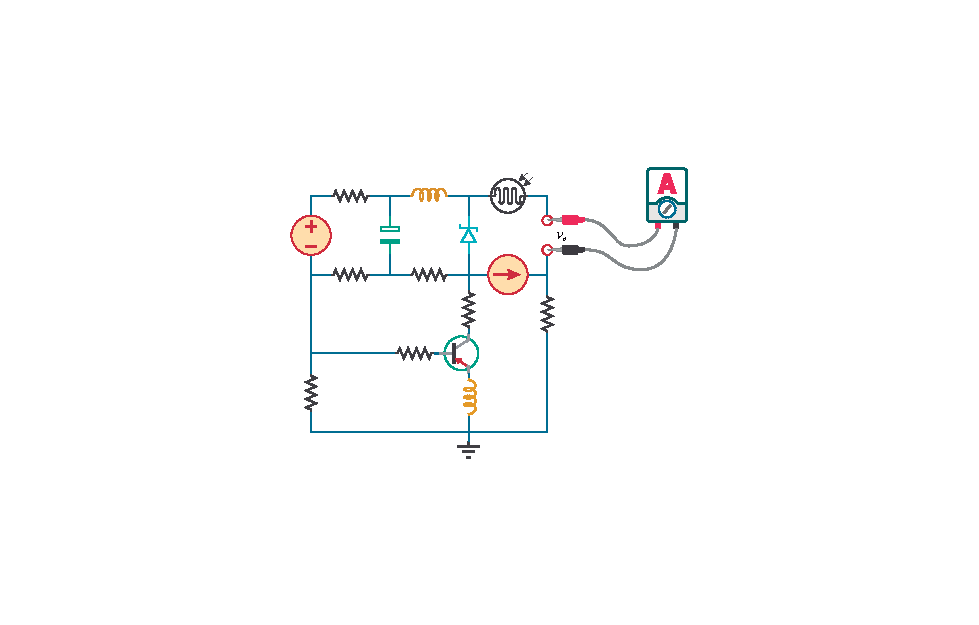
\includegraphics{04-Figuras/Template-figura-A4-ABNT}

Fonte: fonte

\label{figura:figura-exemplo}

\end{figure}

% ------------------------------------------------------------------------------------------------

At vero eos et accusamus et iusto odio dignissimos ducimus qui blanditiis praesentium voluptatum deleniti atque corrupti quos dolores et quas molestias excepturi sint occaecati cupiditate non provident, similique sunt in culpa qui officia deserunt mollitia animi, id est laborum et dolorum fuga. Et harum quidem rerum facilis est et expedita distinctio. Nam libero tempore, cum soluta nobis est eligendi optio cumque nihil impedit quo minus id quod maxime placeat facere possimus, omnis voluptas assumenda est, omnis dolor repellendus. Temporibus autem quibusdam et aut officiis debitis aut rerum necessitatibus saepe eveniet ut et voluptates repudiandae sint et molestiae non recusandae. Itaque earum rerum hic tenetur a sapiente delectus, ut aut reiciendis voluptatibus maiores alias consequatur aut perferendis doloribus asperiores repellat.

At vero eos et accusamus et iusto odio dignissimos ducimus qui blanditiis praesentium voluptatum deleniti atque corrupti quos dolores et quas molestias excepturi sint occaecati cupiditate non provident, similique sunt in culpa qui officia deserunt mollitia animi, id est laborum et dolorum fuga. Et harum quidem rerum facilis est et expedita distinctio. Nam libero tempore, cum soluta nobis est eligendi optio cumque nihil impedit quo minus id quod maxime placeat facere possimus, omnis voluptas assumenda est, omnis dolor repellendus. Temporibus autem quibusdam et aut officiis debitis aut rerum necessitatibus saepe eveniet ut et voluptates repudiandae sint et molestiae non recusandae. Itaque earum rerum hic tenetur a sapiente delectus, ut aut reiciendis voluptatibus maiores alias consequatur aut perferendis doloribus asperiores repellat.


\section{Motivação}

At vero eos et accusamus et iusto odio dignissimos ducimus qui blanditiis praesentium voluptatum deleniti atque corrupti quos dolores et quas molestias excepturi sint occaecati cupiditate non provident, similique sunt in culpa qui officia deserunt mollitia animi, id est laborum et dolorum fuga. Et harum quidem rerum facilis est et expedita distinctio. Nam libero tempore, cum soluta nobis est eligendi optio cumque nihil impedit quo minus id quod maxime placeat facere possimus, omnis voluptas assumenda est, omnis dolor repellendus. Temporibus autem quibusdam et aut officiis debitis aut rerum necessitatibus saepe eveniet ut et voluptates repudiandae sint et molestiae non recusandae. Itaque earum rerum hic tenetur a sapiente delectus, ut aut reiciendis voluptatibus maiores alias consequatur aut perferendis doloribus asperiores repellat.

At vero eos et accusamus et iusto odio dignissimos ducimus qui blanditiis praesentium voluptatum deleniti atque corrupti quos dolores et quas molestias excepturi sint occaecati cupiditate non provident, similique sunt in culpa qui officia deserunt mollitia animi, id est laborum et dolorum fuga. Et harum quidem rerum facilis est et expedita distinctio. Nam libero tempore, cum soluta nobis est eligendi optio cumque nihil impedit quo minus id quod maxime placeat facere possimus, omnis voluptas assumenda est, omnis dolor repellendus. Temporibus autem quibusdam et aut officiis debitis aut rerum necessitatibus saepe eveniet ut et voluptates repudiandae sint et molestiae non recusandae. Itaque earum rerum hic tenetur a sapiente delectus, ut aut reiciendis voluptatibus maiores alias consequatur aut perferendis doloribus asperiores repellat.


\section{Objetivos}

At vero eos et accusamus et iusto odio dignissimos ducimus qui blanditiis praesentium voluptatum deleniti atque corrupti quos dolores et quas molestias excepturi sint occaecati cupiditate non provident, similique sunt in culpa qui officia deserunt mollitia animi, id est laborum et dolorum fuga. Et harum quidem rerum facilis est et expedita distinctio. Nam libero tempore, cum soluta nobis est eligendi optio cumque nihil impedit quo minus id quod maxime placeat facere possimus, omnis voluptas assumenda est, omnis dolor repellendus. Temporibus autem quibusdam et aut officiis debitis aut rerum necessitatibus saepe eveniet ut et voluptates repudiandae sint et molestiae non recusandae. Itaque earum rerum hic tenetur a sapiente delectus, ut aut reiciendis voluptatibus maiores alias consequatur aut perferendis doloribus asperiores repellat.

At vero eos et accusamus et iusto odio dignissimos ducimus qui blanditiis praesentium voluptatum deleniti atque corrupti quos dolores et quas molestias excepturi sint occaecati cupiditate non provident, similique sunt in culpa qui officia deserunt mollitia animi, id est laborum et dolorum fuga. Et harum quidem rerum facilis est et expedita distinctio. Nam libero tempore, cum soluta nobis est eligendi optio cumque nihil impedit quo minus id quod maxime placeat facere possimus, omnis voluptas assumenda est, omnis dolor repellendus. Temporibus autem quibusdam et aut officiis debitis aut rerum necessitatibus saepe eveniet ut et voluptates repudiandae sint et molestiae non recusandae. Itaque earum rerum hic tenetur a sapiente delectus, ut aut reiciendis voluptatibus maiores alias consequatur aut perferendis doloribus asperiores repellat.


\section{Materiais e Métodos}

At vero eos et accusamus et iusto odio dignissimos ducimus qui blanditiis praesentium voluptatum deleniti atque corrupti quos dolores et quas molestias excepturi sint occaecati cupiditate non provident, similique sunt in culpa qui officia deserunt mollitia animi, id est laborum et dolorum fuga. Et harum quidem rerum facilis est et expedita distinctio. Nam libero tempore, cum soluta nobis est eligendi optio cumque nihil impedit quo minus id quod maxime placeat facere possimus, omnis voluptas assumenda est, omnis dolor repellendus. Temporibus autem quibusdam et aut officiis debitis aut rerum necessitatibus saepe eveniet ut et voluptates repudiandae sint et molestiae non recusandae. Itaque earum rerum hic tenetur a sapiente delectus, ut aut reiciendis voluptatibus maiores alias consequatur aut perferendis doloribus asperiores repellat.


\section{Organização do Trabalho}

At vero eos et accusamus et iusto odio dignissimos ducimus qui blanditiis praesentium voluptatum deleniti atque corrupti quos dolores et quas molestias excepturi sint occaecati cupiditate non provident, similique sunt in culpa qui officia deserunt mollitia animi, id est laborum et dolorum fuga. Et harum quidem rerum facilis est et expedita distinctio. Nam libero tempore, cum soluta nobis est eligendi optio cumque nihil impedit quo minus id quod maxime placeat facere possimus, omnis voluptas assumenda est, omnis dolor repellendus. Temporibus autem quibusdam et aut officiis debitis aut rerum necessitatibus saepe eveniet ut et voluptates repudiandae sint et molestiae non recusandae. Itaque earum rerum hic tenetur a sapiente delectus, ut aut reiciendis voluptatibus maiores alias consequatur aut perferendis doloribus asperiores repellat.					%-> Introdução
\chapter{Revisão Bibliográfica}



\section{Nanofotônica}

Parágrafo.

\section{Dispositivos Fotônicos}

Parágrafo.



\section{Machine Learning}

Parágrafo.

\subsection{Redes Neurais Artificiais}

Parágrafo.


\subsection{Algorítmo de Aprendizagem}

Parágrafo.		%-> Revisão Bibliográfica
\chapter{Método Proposto}      \label{Metodo Proposto}

Otimizar os dispositivos nanofotônicos requer um trabalho de análise muito cuidadoso e assertivo. Cada simulação computacional pode demandar um tempo.

\section{Visão Geral}

Morbi a metus. Phasellus enim erat, vestibulum vel, aliquam a, posuere eu, velit. Nullam sapien sem, ornare ac, nonummy non, lobortis a, enim. Nunc tincidunt ante vitae massa. Duis ante orci, molestie vitae, vehicula venenatis, tincidunt ac, pede. Nulla accumsan, elit sit amet varius semper, nulla mauris mollis quam, tempor suscipit diam nulla vel leo. Etiam commodo dui eget wisi. Donec iaculis gravida nulla. Donec quis nibh at felis congue commodo. Etiam bibendum elit eget erat.


\section{Descrição do Problema}

Morbi a metus. Phasellus enim erat, vestibulum vel, aliquam a, posuere eu, velit. Nullam sapien sem, ornare ac, nonummy non, lobortis a, enim. Nunc tincidunt ante vitae massa. Duis ante orci, molestie vitae, vehicula venenatis, tincidunt ac, pede. Nulla accumsan, elit sit amet varius semper, nulla mauris mollis quam, tempor suscipit diam nulla vel leo. Etiam commodo dui eget wisi. Donec iaculis gravida nulla. Donec quis nibh at felis congue commodo. Etiam bibendum elit eget erat.


\section{Otimização por Aprendizado Profundo}

Maecenas ipsum velit, consectetuer eu, lobortis ut, dictum at, dui. In rutrum. Sed ac dolor sit amet purus malesuada congue. In laoreet, magna id viverra tincidunt, sem odio bibendum justo, vel imperdiet sapien wisi sed libero. Suspendisse sagittis ultrices augue. Mauris metus. Nunc dapibus tortor vel mi dapibus sollicitudin. Etiam posuere lacus quis dolor. Praesent id justo in neque elementum ultrices. Class aptent taciti sociosqu ad litora torquent per conubia nostra, per inceptos hymenaeos. In convallis. Fusce suscipit libero eget elit. Praesent vitae arcu tempor neque lacinia pretium. Morbi imperdiet, mauris ac auctor dictum, nisl ligula egestas nulla, et sollicitudin sem purus in lacus.

\begin{figure}[H]
    \centering
    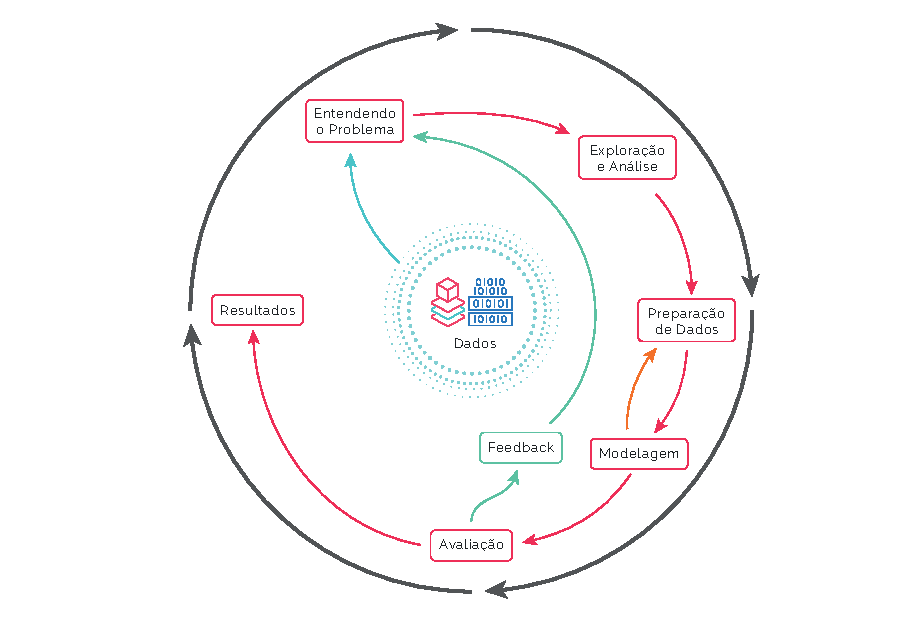
\includegraphics{04-Figuras/DataScienceDutyCicle.eps}
    \caption{Ciclo de trabalho de um projeto em ciência de dados.} \par
    Fonte: do Autor.
    \label{figura: DataScienceDutyCicle}
\end{figure}


\subsection{Construção do Banco de Dados}

O procedimento de otimização por inteligência artificial envolve, primeiramente, coletar os dados do problema e organizá-los em um banco de dados. Estes dados podem ser coletados por meio da API (\textit{Application Programming Interface}, ou ainda em português, Interface de Programação de Aplicativos) que o próprio COMSOL oferece. Uma API permite que aconteça troca de informações entre dois ou mais sistemas. Neste caso, a API \textit{COMSOL LiveLink for MATLAB} permite que o MATLAB possa controlar como as simulações numéricas do COMSOL acontecem, desde o processo de automatizá-las, à triagem desses dados para a construção do banco de dados.

Os dispositivos nanofotônicos são modelados e estudados a partir do software de simulação eletromagnética COMSOL. Nessa etapa, o próprio usuário constrói o dispositivo com as características geométricas e de operação que ele deve ter (como mostrado na Seção \ref{Modelando COMSOL} do Capítulo \ref{Revisao Bibliografica} deste documento).

Uma vez que esse estudo esteja estabelecido, o próximo passo é mapear variáveis que modificam a geometria do dispositivo simetricamente, respeitando assim a simetria do problema conforme estabelecido pela \textit{Teoria de Grupos} (ver Seção \ref{Embasamento Teorico} do Capítulo \ref{Revisao Bibliografica}). A Fig. mostra como esse processo de mapeamento é implementado. 

As mesmas variáveis que modificam simetricamente a geometria do dispositivo são usadas em um \textit{script} no MATLAB. A ideia por trás desse script é automatizar as simulações em loops de execução. A cada execução o matlab atribui valores randômicos para essas variáveis. Em termos práticos, isso significa que cada simulação de dispositivo terá uma geometria diferente para simular.


Ao final de uma simulação, os dados randômicos de geometria e a respectiva resposta em frequência são exportados em arquivos com a extensão \textit{.txt} e amarzenados em uma pasta no computadoor em um diretório definido também no mesmo script do MATLAB.

\begin{figure}[H]
    \centering
    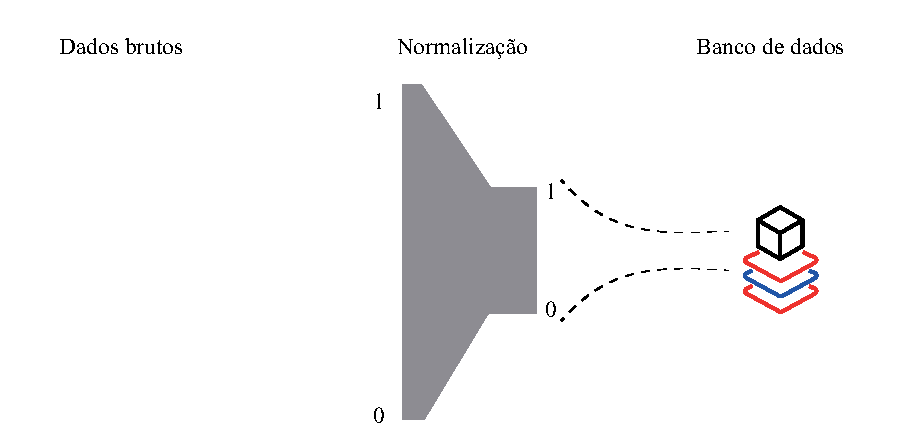
\includegraphics{04-Figuras/DatasetMounting.eps}
    \caption{Procedimento de contrução do dataset.} \par
    Fonte: do Autor.
    \label{figura: DatasetMounting}
\end{figure}

Foi desenvolvido também um outro script no MATLAB que é resposável por ler os dados gerados pelas simulações automatizadas. A função desse \textit{script} é ler todos os arquivos de simulação que foram gerados e montar o banco de dados em um único arquivo, onde os dados estão organizados de maneira sequencial (conforme o loop de simulação) e normalizados no intervalo $0\dotso 1$ (o procedimento de normalização está explicado na Seção deste Capítulo).

\begin{figure}[H]
    \centering
    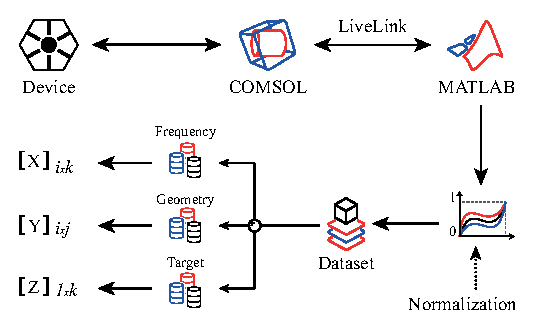
\includegraphics{04-Figuras/DatasetBuilding.eps}
    \caption{Procedimento de contrução do dataset.} \par
    Fonte: do Autor.
    \label{figura: DatasetBuilding}
\end{figure}

Assim, nessa etapa, são gerados três arquivos na extensão \textit{.csv}, cada qual entendidos como tensores, a saber:

\begin{itemize}
	\item \textbf{Resposta em Frequência} -- definido pelo tensor $[X]$, compreende as amplitudes discretizadas da resposta, sequenciadas linha-a-linha.
	\item \textbf{Geometria} -- definido pelo tensor $[Y]$, compreende os dados randômicos usados para modificar a geometria.
	\item \textbf{Espectro Desejado} -- definido pelo tensor $[Z]$, compreende à resposta em frequência desejada para o dispositivo definido pelo próprio projetista do dispositivo.
\end{itemize}









\begin{equation}
\label{eq:tensorY}
\mathbf{[Y]_{i,j}} =
\begin{bmatrix}
y_{1_{[1,1]}} & y_{2_{[1,2]}} & \cdots & y_{j_{[1,j]}}\\
y_{1_{[2,1]}} & y_{2_{[2,2]}} & \cdots & y_{j_{[2,j]}}\\
\vdots  & \vdots  & \ddots & \vdots\\
y_{1_{[i,1]}} & y_{2_{[i,2]}} & \cdots & y_{j_{[i,j]}}
\end{bmatrix},
\end{equation}

\noindent
where $j$ is the total number of the variables that modify the device's geometry and $i$ refers to the number of samples, i. e., the number of instances. The same reasoning applies to the construction of the frequency response dataset, whose are grouped into a tensor defined as:

\begin{equation}
\label{eq:tensorX}
\mathbf{[X]_{i,k}} =
\begin{bmatrix}
x_{1_{[1,1]}} & x_{2_{[1,2]}} & \cdots & x_{k_{[1,k]}}\\
x_{1_{[2,1]}} & x_{2_{[2,2]}} & \cdots & x_{k_{[1,k]}}\\
\vdots  & \vdots  & \ddots & \vdots\\
x_{1_{[i,1]}} & x_{2_{[i,2]}} & \cdots & x_{k_{[i,k]}}
\end{bmatrix}.
\end{equation}

Note that the instance number \textit{i} must be the same length for $\mathbf{[X]}$ and $\mathbf{[Y]}$, because geometry and frequency response need to be related. And, finally, the target frequency response is defined as a tensor:

\begin{equation}
\label{eq:tensorZ}
\mathbf{[Z]_{1,k}} =
\begin{bmatrix}
z_{1_{[1,1]}} & z_{2_{[1,2]}} & \cdots & z_{k_{[1,k]}}\\
\end{bmatrix}.
\end{equation}

As mentioned above, the tensor $\mathbf{[Z]}$ was made considering the ideal characteristics for the frequency response.


\subsection{Rede Neural Profunda}

A Rede Neural Profunda (sigla DNN, em inglês) foi desenvolvida na linguagem de programação Python com a \textit{framekork} Tensorflow. 

\subsection{Treinamento e Predição}

We train the DNN using Adam as an optimization algorithm, with a mean squared error (MSE) as a cost function. The training procedure is made by minimizing the cost function $C$, as shown in Eq. \ref{eq:costFunction}.

\begin{equation}
\label{eq:costFunction}
C = \frac{1}{n}\sum_{i=1}^{n}\left ( Y_{i} - \hat{Y}_{i} \right )^{2}.
\end{equation}


\subsection{Procedimento de Otimização}

Aenean placerat. In vulputate urna eu arcu. Aliquam erat volutpat. Suspendisse potenti. Morbi mattis felis at nunc. Duis viverra diam non justo. In nisl. Nullam sit amet magna in magna gravida vehicula. Mauris tincidunt sem sed arcu. Nunc posuere. Nullam lectus justo, vulputate eget, mollis sed, tempor sed, magna. Cum sociis natoque penatibus et magnis dis parturient montes, nascetur ridiculus mus. Etiam neque. Curabitur ligula sapien, pulvinar a, vestibulum quis, facilisis vel, sapien. Nullam eget nisl. Donec vitae arcu.

\begin{figure}[H]
    \centering
    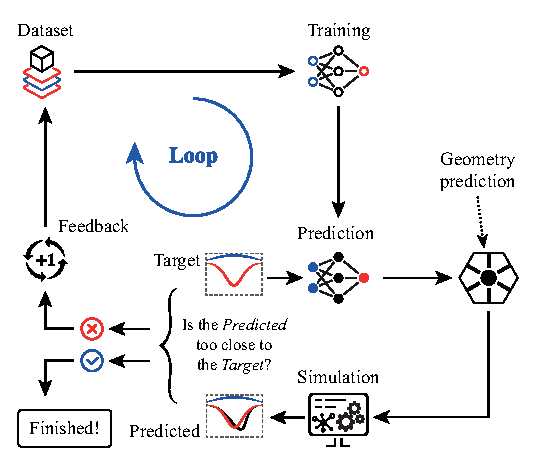
\includegraphics{04-Figuras/OptimizationAlgorithm.eps}
    \caption{Algorítmo de otimização.} \par
    Fonte: do Autor.
    \label{figura: OptimizationAlgorithm}
\end{figure}

Nam quis nulla. Integer malesuada. In in enim a arcu imperdiet malesuada. Sed vel lectus. Donec odio urna, tempus molestie, porttitor ut, iaculis quis, sem. Phasellus rhoncus. Aenean id metus id velit ullamcorper pulvinar. Vestibulum fermentum tortor id mi. Pellentesque ipsum. Nulla non arcu lacinia neque faucibus fringilla. Nulla non lectus sed nisl molestie malesuada. Proin in tellus sit amet nibh dignissim sagittis. Vivamus luctus egestas leo. Maecenas sollicitudin. Nullam rhoncus aliquam metus. Etiam egestas wisi a erat.


\section{Aplicação em Cristal Fotônico 2D}

Maecenas ipsum velit, consectetuer eu, lobortis ut, dictum at, dui. In rutrum. Sed ac dolor sit amet purus malesuada congue. In laoreet, magna id viverra tincidunt, sem odio bibendum justo, vel imperdiet sapien wisi sed libero. Suspendisse sagittis ultrices augue. Mauris metus. Nunc dapibus tortor vel mi dapibus sollicitudin. Etiam posuere lacus quis dolor. Praesent id justo in neque elementum ultrices. Class aptent taciti sociosqu ad litora torquent per conubia nostra, per inceptos hymenaeos. In convallis. Fusce suscipit libero eget elit. Praesent vitae arcu tempor neque lacinia pretium. Morbi imperdiet, mauris ac auctor dictum, nisl ligula egestas nulla, et sollicitudin sem purus in lacus.

\subsection{Princípio de Funcionamento}

Morbi a metus. Phasellus enim erat, vestibulum vel, aliquam a, posuere eu, velit. Nullam sapien sem, ornare ac, nonummy non, lobortis a, enim. Nunc tincidunt ante vitae massa. Duis ante orci, molestie vitae, vehicula venenatis, tincidunt ac, pede. Nulla accumsan, elit sit amet varius semper, nulla mauris mollis quam, tempor suscipit diam nulla vel leo. Etiam commodo dui eget wisi. Donec iaculis gravida nulla. Donec quis nibh at felis congue commodo. Etiam bibendum elit eget erat.

\begin{figure}[H]
    \centering
    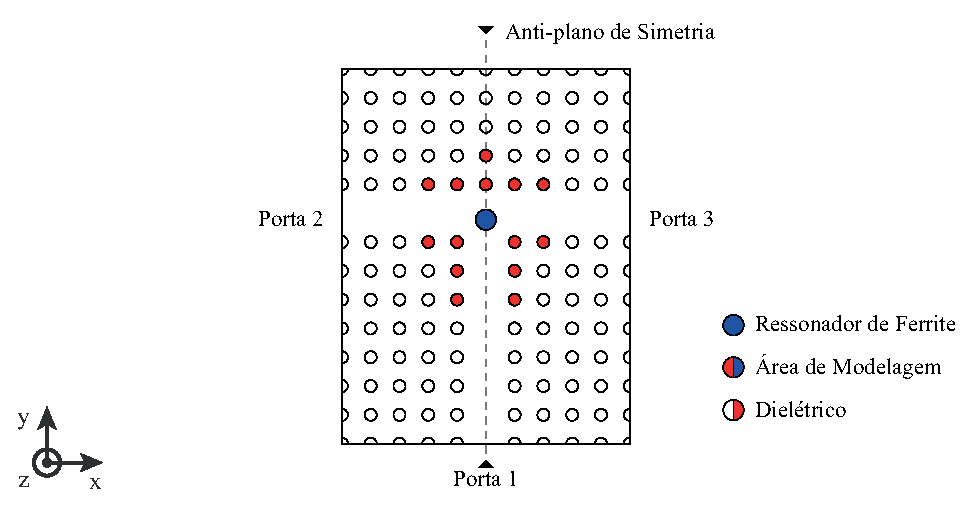
\includegraphics{04-Figuras/PhotonicCrystal.eps}
    \caption{Geometria do cristal fotônico.} \par
    Fonte: do Autor.
    \label{figura: PhotonicCrystal}
\end{figure}

\subsection{Ressonador Dipolo}

Nam quis nulla. Integer malesuada. In in enim a arcu imperdiet malesuada. Sed vel lectus. Donec odio urna, tempus molestie, porttitor ut, iaculis quis, sem. Phasellus rhoncus. Aenean id metus id velit ullamcorper pulvinar. Vestibulum fermentum tortor id mi. Pellentesque ipsum. Nulla non arcu lacinia neque faucibus fringilla. Nulla non lectus sed nisl molestie malesuada. Proin in tellus sit amet nibh dignissim sagittis. Vivamus luctus egestas leo. Maecenas sollicitudin. Nullam rhoncus aliquam metus. Etiam egestas wisi a erat.


\subsection{Ressonador Quadripolo}

Maecenas ipsum velit, consectetuer eu, lobortis ut, dictum at, dui. In rutrum. Sed ac dolor sit amet purus malesuada congue. In laoreet, magna id viverra tincidunt, sem odio bibendum justo, vel imperdiet sapien wisi sed libero. Suspendisse sagittis ultrices augue. Mauris metus. Nunc dapibus tortor vel mi dapibus sollicitudin. Etiam posuere lacus quis dolor. Praesent id justo in neque elementum ultrices. Class aptent taciti sociosqu ad litora torquent per conubia nostra, per inceptos hymenaeos. In convallis. Fusce suscipit libero eget elit. Praesent vitae arcu tempor neque lacinia pretium. Morbi imperdiet, mauris ac auctor dictum, nisl ligula egestas nulla, et sollicitudin sem purus in lacus.
			%-> Desenvolvimento
\chapter{Resultados}



\section{Objetivos}

Parágrafo.

\section{Avaliação da Função Custo}

Parágrafo.					%-> Resultados
\chapter{Considerações Finais}      \label{Consideracoes Finais}

\section{Discussão}

No âmbito da modelagem inversa, não é sempre garantido que haverá uma solução para o problema, isto é, que tenha de fato uma resposta em frequência com parâmetros de operação desejados. O problema associado é o da \textit{não-unicidade} da resposta eletromagnética de muitos dispositivos. Nesse caso, duas ou mais configurações de geometria podem ocasionar na mesma resposta de campo (ou resposta em frequência). Esse problema, inclusive, foi discutido em \cite{liu2018training} e previamente comentado no Capítulo \ref{Introducao} deste trabalho. Deve-se pontuar que, apesar dessa temática não ser abordada na metodologia deste trabalho, é um problema que deve-se considerar para trabalhos futuros.

Outra discussão, é o fato de o banco de dados não ser estático, isto é, há um incremento no número de instâncias à medida que o algorítimo é executado. Por este motivo foi feito o procedimento de gerar um \textit{banco de dados inicial} para posteriormente escolher a arquitetura de rede e, finalmente, continuar com o trabalho.

Durante o Capítulo \ref{Metodo Proposto}, foi mencionado que a resposta em frequência foi discretizada em 51 pontos. Essa escolha se deu por conta da quantidade de informações que serão repassadas à rede. Quanto mais pontos as curvas forem discretizadas, maior será a dimensão da camada de entrada, mais dados serão processados, o que irá requerer mais tempo. Com menos pontos de discretização, certamente será um processamento mais rápido, entretanto, poderá faltar informações valiosas para o aprendizado, tornando o modelo menos preciso. Desta forma, 51 foi uma escolha considerada ótima entre essas questões discutidas.

A escolha de uma camada de \textit{pré-processamento} na arquitetura da rede neural profunda foi feita com base no trabalho discutido em \cite{malkiel2017deep}. Quando implementada, foi verificado um melhoramento na precisão da rede neural profunda. A camada de pré-processamento irá tratar cada curva da resposta em frequência de forma independente e paralela (é como se cada curva tivesse a sua própria rede neural), para então serem alimentadas na rede sequencial.

Os resultados de ambos circuladores baseado em cristal fotônico foi alcançado em até 3 semanas após a implementação do método de otimização e modelagem inversa abordado no presente trabalho. Em contrapartida, em métodos convencionais, esse tempo normalmente é de alguns meses, podendo chegar a alguns anos.

\newpage
\section{Conclusão}

Neste \imprimirtipotrabalho, foi apresentado um procedimento de otimização e modelagem inversa de dispositivos nanofotônicos com o uso de algoritmos em \textit{machine learning}. Os dispositivos nanofotônicos de hoje dependem cada vez mais de nanoestruturas complexas para realizar funcionalidades sofisticadas. À medida que essa complexidade estrutural aumenta, os processos de projeto se tornam mais desafiadores.

Para ambos os dispositivos baseados em Cristal Fotônico, os resultados foram muito promissores. Conforme relatado no presente trabalho, a caracterização da resposta em frequência de ambos dispositivos ficaram próximas da resposta em frequência desejada, respeitando características de projeto cruciais, como o alinhamento das curvas dos parâmetros-S em ressonância na frequência central de operação dos dispositivos. Para os dispositivos divisores de potência baseados em grafeno (ver Apêndice \ref{Apendice}), os resultados ainda não foram promissores e, certamente, requerem uma nova abordagem metodológica (como as demais abordagens de alto DOF discutidas na Seção \ref{Trabalhos Relacionados} do Capítulo \ref{Introducao}). Também é importante considerar que existe a possibilidade, seja pela própria característica eletromagnética do dispositivo, de não existir uma resposta em frequência com características ótimas de operação e, portanto, não existir uma convergência para a modelagem inversa da estrutura analisada.

De uma forma geral, o método desenvolvido se apresentou promissor para a caracterização de nanoestruturas, pois as redes neurais profundas conseguem relacionar muito bem problemas multivariáveis e não-lineares, o que na condição da análise humana através de um processo intuitivo e empírico, torna-se uma tarefa bastante demorada e desafiadora.

O presente trabalho teve como principal objetivo demonstrar ao leitor quais passos e análises seguir para a modelagem inversa de estruturas. Ressalta-se, portanto, que essa metodologia pode ser aplicada a qualquer problema que envolva o \textit{design} de estruturas, independentemente da escala do problema. O uso da API \textit{Comsol LiveLink For Matlab} também é uma ferramenta de projeto crucial, pois automatiza e integra vários processos.

Nota-se que o poder da Inteligência Artificial, em geral, e as abordagens de Aprendizagem Profunda, em particular, têm implicações de grande impacto no campo da nanotecnologia e nanofotônica, como demonstrado no presente trabalho de \textit\imprimirtitulo, e brevemente discutido em trabalhos relacionados na Introdução deste documento. Esse avanço não se restringe somente à tecnologia, mas atinge também as empresas, os setores públicos, o mercado financeiro, etc. Esse novo olhar para a análise dos dados permite tornar os sistemas cada vez mais robustos e eficientes.


\newpage
\section{Sugestões Para Trabalhos Futuros}

Para trabalhos futuros, são sugeríveis os estudos:

\begin{itemize}
    \item Desenvolver uma abordagem de modelagem inversa em torno de Redes Neurais Adversárias Generativas (\textit{Generative Adversarial Network (GAN)}).
    \item Averiguar o uso de Redes Neurais Convolucionais (\textit{Convolutional Neural Networks (CNN)}).
\end{itemize}


\section{Trabalhos Desenvolvidos}

O presente \imprimirtipotrabalho\ teve contribuição aos seguintes trabalhos:

\begin{itemize}
    \item V. Dmitriev, L. Martins, G. Portela and L. H. Assunção, \textit{"Quadrupole resonator mode versus dipole one in photonic crystal ferrite circulators"}, Photonics and Nanostructures - Fundamentals and Applications, (2021). \cite{DMITRIEV2021100954}
    \item V. Dmitriev, G. Portela, F. Nobre, W. Castro and L. H. Assunção, \textit{"Nonreciprocal Dynamically Tunable Power Dividers By Three (1x3) Based on Graphene for Terahertz Region"}, Optics Communications, (2021) \cite{Dmitriev2021Nonreciprocal}.
\end{itemize}

Para fins de consulta do leitor, o desenvolvimento de todos os \textit{scripts} podem ser consultado no repositório \textit{GitHub}:

\begin{itemize}
    \item Dispositivos baseados em cristal fotônico \cite{luizheinrich2021PhC}.
    \item Dispositivos baseados em Grafeno \cite{luizheinrich2021Graphene}.
\end{itemize}
		%-> Considerações Finais


% ELEMENTOS PÓS-TEXTUAIS =========================================================================

\postextual
%=================================================================================================
%=							       		    REFERÊNCIAS											 =
%=================================================================================================


\chapter{Referências Bibliográficas}
\bibliography{Bibliografia.bib}
			%-> Referências
\chapter{Glossário}

				%-> Glossário
\chapter{Apêndice}

\section{Apêndice A}

vgvgvcfgc

\newpage

\section{Apêndice B}

 vghvygvgy				%-> Apêndice
\chapter{Anexos}

\section{Anexo A}

vgvgvcfgc



\newpage %====================================================================================

\section{Anexo B}

 vghvygvgy					%-> Anexo
%=================================================================================================
%=							       		       CAPA							     			 	 =
%=================================================================================================


\chapter{Índice}

\printindex					%-> Índice


%=================================================================================================

\end{document}